\chapter{Basics on classification}

\begin{remark}{Outline}
\todo{outline}
In this chapter, we present the well-known family of \textit{random forests}
methods. In Section~\ref{sec:4:bias-variance}, we first describe the bias-variance
decomposition of the prediction error and then present, in
Section~\ref{sec:4:ensemble}, how aggregating randomized models through
ensembles reduces the prediction error by decreasing the variance term in this
decomposition. In Section~\ref{sec:4:random-forests}, we revisit random forests
and its variants and study how randomness introduced into the decision trees
reduces prediction errors by decorrelating the decision
trees in the ensemble. Properties and features of random forests are then outlined
in Section~\ref{sec:4:features} while their consistency
is finally explored in Section~\ref{sec:4:consistency}.
\end{remark}


\section{Classification models}
In machine learning, classification refers to attempt to identify to which of a set of classes a 
new example belongs, based on learning from examples whose class membership is known. The most 
important point about classification is that for each example only one know class is possible, 
making this a discrete problem.

A classification, task begins with a training set in which the class of a set of examples is know. 
For example, a classification model that predicts credit card fraud, is developed by analyzing 
many observed credit transactions over a period of time. The class in this case is a variable which 
indicates for each example whether or not the transaction was o not a fraud. Also, the predictors 
or features, are the transaction attributes like place, amount and time.

Then, during the training process, a classification algorithm finds the patterns and relationships 
between the values of the features and the values of the target class, Different algorithms use 
different methods and techniques to estimate the relationships. Afterwards, these relationships are 
summarized in a model that is able to make predictions on new sets of data.

In \figurename{ \ref{fig:ch2:1}}, a set of examples from two different classes is shown. The an 
algorithm is learn in order to separate between the two classes, positive and negative. In this 
example, the algorithm attempts to make a classification that separates the better between the 
classes. However, it is expected that in not all cases a perfect separation is obtain. 
\todo{expand}

Formally, a classification algorithm is a function that map ... \todo{add definitions, sets}

\begin{figure}[!t]
\centering
\subfloat[]{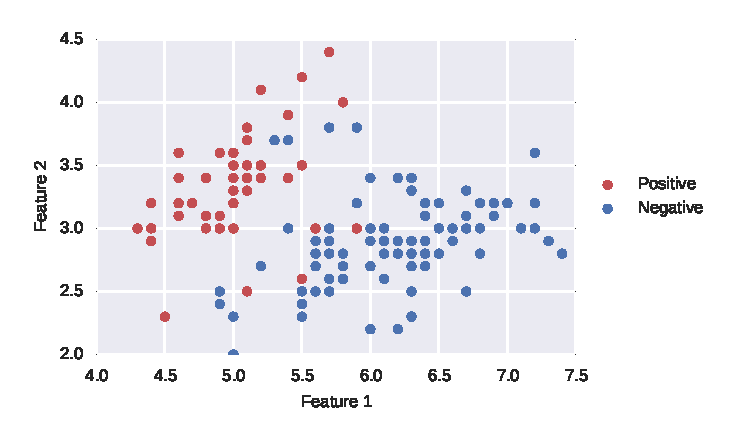
\includegraphics{ch2_fig1a}\label{fig:ch2:1a}}
\\
\subfloat[]{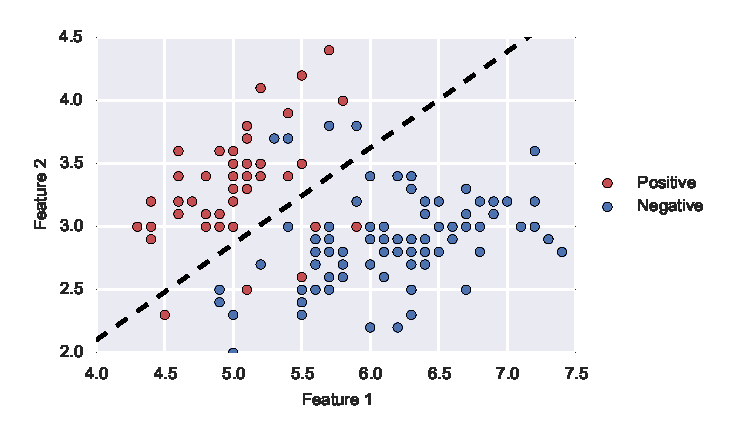
\includegraphics{ch2_fig1b}\label{fig:ch2:1b}}
\caption{Example of a classification algorithm. Using a set of examples from two classes, a 
	classification algorithm is learn in order to separate between the positives and the negatives. }
\label{fig:ch2:1}
\end{figure} 

	
\begin{remark}{Classification examples}
Classification algorithms are widely used across a variety of domains. For example in the 
medical field, models have been used for making predictions about tumors, probability 
of a disease, selecting the right drug for a particular patient, and estimating the probability of 
relapsing, among others \citep{Herland2014}. In the financial sector, classification models have 
been successfully applied for fraud detection, credit scoring, portfolio management and algorithmic 
trading. Also, in marketing, several models are being currently used for churn modeling, customer 
targeting, behavior prediction and direct marketing \citep{Baesens2014}. Additionally, in many 
other emerging applications such as terrorism prevention, malware detection, computer security, 
energy consumption prediction, spam classification, and others \citep{Kriegel2007}.
\end{remark}

\section{Performance measures}

When constructing a classification algorithm, the true class of the training examples is known. 
Therefore, evaluating the error of a model is as simply as counting the number of times an example 
is misclassified and divide it by the number of examples.

\todo{eq error}

Moreover the accuracy is defined as the percentage of times the algorithm made the correct 
prediction

\todo{eq acc}

However, just knowing these statistics is not enough to make decisions, as in many applications is 
important to know where the errors are coming from. In particular, the misclassified examples may 
belong only to one class, which may give interesting insights about the problem.
A way to observe the different errors is by looking to the confusion matrix.
As shown in \tablename{ \ref{tab:ch2:1}}, 
\todo{how to calculate TP, FP...}

	\begin{table}[!t]
		\centering
    \begin{tabular}{c|c|c}
      \multicolumn{3}{c}{}\\
			\multicolumn{1}{c|}{}  & Actual Positive& Actual Negative \\
			\multicolumn{1}{c|}{} & $y=1$& $y=0$ \\
			\hline
			Predicted Positive 		& \multirow{ 2}{*}{True Positive ($TP$)} & \multirow{ 
			2}{*}{False Positive ($FP$)} \\
			$c=1$ & &\\
			\hline
			Predicted Negative  	& \multirow{ 2}{*}{False Negative ($FN$)} & \multirow{ 
			2}{*}{True Positive ($TN$)} \\
			$c=0$ & &\\
		\end{tabular}
		\caption{Classification confusion matrix}
		\label{tab:ch2:1}
  \end{table}  

  	From this table several statistics are extracted. In particular:
	\begin{itemize}
		\item Recall = $\frac{TP}{TP+FN}$
		\item Precision = $\frac{TP}{TP+FP}$
		\item $F_1Score = 2\frac{Precision \cdot Recall}{Precision + Recall}$
	\end{itemize}


  
  	\begin{table}[!t]
		\centering
    \begin{tabular}{c|c|c}
      \multicolumn{3}{c}{}\\
			\multicolumn{1}{c|}{}  & Actual Positive& Actual Negative \\
			\multicolumn{1}{c|}{} & $y=1$& $y=0$ \\
			\hline
			Predicted Positive 		& \multirow{ 2}{*}{36} & \multirow{ 
			2}{*}{4} \\
			$c=1$ & &\\
			\hline
			Predicted Negative  	& \multirow{ 2}{*}{5} & \multirow{ 
			2}{*}{68} \\
			$c=0$ & &\\
		\end{tabular}
		\caption{Confusion matrix of the toy example}
		\label{tab:ch2:2}
  \end{table}  
  
  Calculating the different statistics for this example
  	\begin{itemize}
  	\item Error = $\frac{4+9}{36+4+9+68}=8\%$
		\item Recall = $\frac{TP}{TP+FN}$
		\item Precision = $\frac{TP}{TP+FP}$
		\item $F_1Score = 2\frac{Precision \cdot Recall}{Precision + Recall}$
	\end{itemize}
	
	In order to make a comparison, using the same example toy set, a new algorithm is learn. This 
time the algorithm made the correct prediction more often as shown in \figurename{ \ref{fig:ch2:2}}.

\begin{figure}[t!]
	\centering
	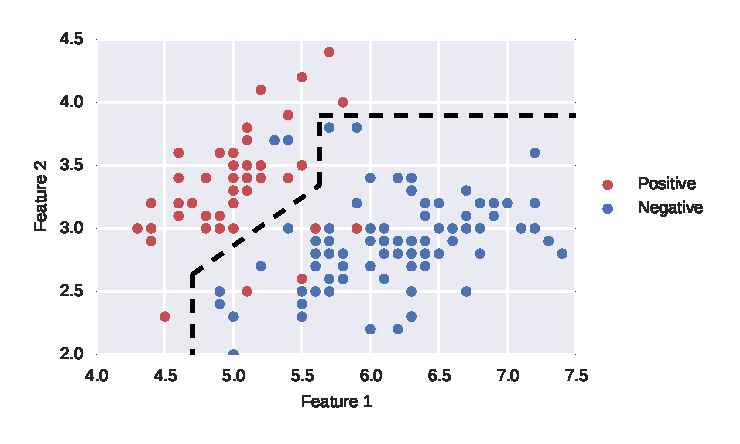
\includegraphics{ch2_fig2}
	\caption{Example of a classification algorithm. Using a set of examples from two classes, a 
	classification algorithm is learn in order to separate between the positives and the negatives. }
	\label{fig:ch2:2}
\end{figure}

    	\begin{table}[!t]
		\centering
    \begin{tabular}{c|c|c}
      \multicolumn{3}{c}{}\\
			\multicolumn{1}{c|}{}  & Actual Positive& Actual Negative \\
			\multicolumn{1}{c|}{} & $y=1$& $y=0$ \\
			\hline
			Predicted Positive 		& \multirow{ 2}{*}{37} & \multirow{ 
			2}{*}{2} \\
			$c=1$ & &\\
			\hline
			Predicted Negative  	& \multirow{ 2}{*}{4} & \multirow{ 
			2}{*}{70} \\
			$c=0$ & &\\
		\end{tabular}
		\caption{Confusion matrix of the toy example}
		\label{tab:ch2:2}
  \end{table}  
  Error = 5.31\%
  
\section{Families of binary classifiers}
\subsection{Linear models}
\subsection{Decision tree models}
\subsection{Neural networks}
\subsection{Suport vector machines}
\subsection{Ensemble based classifiers}
\section{Sampling}
\subsection{Under/over sampling}
\subsection{SMOTE}